\documentclass {article}

\usepackage[utf8]{inputenc}
\usepackage{graphicx}
\usepackage{listings}
\usepackage{color}
\usepackage{float}
\usepackage{multicol}

\definecolor{dkgreen}{rgb}{0,0.6,0}
\definecolor{gray}{rgb}{0.5,0.5,0.5}
\definecolor{mauve}{rgb}{0.58,0,0.82}

\lstset{frame=tb,
    language=C,
    aboveskip=3mm,
    belowskip=3mm,
    showstringspaces=false,
    columns=flexible,
    basicstyle={\small\ttfamily},
    numbers=left,
    numberstyle=\tiny\color{gray},
    keywordstyle=\color{blue},
    commentstyle=\color{dkgreen},
    stringstyle=\color{mauve},
    breaklines=true,
    breakatwhitespace=true,
    tabsize=3
}


\title{Laboratory project report M1\\
Parallel programming for neural networks}
\date{\today}
\author{Djahid ABDELMOUMENE\\
\textit{Encadrant technique:}Philippe GAUSSIER\\
Université de Cergy-Pontoise   ETIS}

\begin{document}
\maketitle
\newpage
\tableofcontents
\newpage
\section{Introduction}
As processors get faster and faster than memory access times, optimisations
start to become necessary in order to utilize the CPU to its full capacity,
this is especially true when trying to write parallel code, since memory access
bottlenecks can throttle the performance greatly, because the access to memory
can't be parallelized which causes race conditions to occur, rendering the
parallel code useless. To avoid this problem the parallel code must utilize the
cache or some sort of secondary SRAM that allows faster access times at the
cost of its storage capacity, which is usually tolerable using some techniques
that will be discussed later on.\\

The main problem addressed here is the optimisation of a neural network simulator
called 'promethe'. the main objective is to use parallel programming to scale up
the performance of the simulator, as well as solve memory access bottlenecks that
are hindering the parallelization of the code.

\section{optimisation techniques}
In this section we review some optimisation techniques that are used to
increase the locality of memory use, that is, increase the reuse of values
loaded into the cache. We'll also see the syntax of OpenMP parallelization and
its effects on the performance.\\

To view these techniques well try to optimize matrix multiplication of two
$N\times N$ matrices in C, We will be sticking to the naive algorithm with
a complexity of $\mathcal{O}(n^3)$.


\subsection{Naive algorithm}
As a baseline for the performance comparison we'll take the naive version of
the matrix multiplication as shown here:

\begin{lstlisting}
for(i=0; i<N; i++) {
    for(j=0; j<N; j++) { 
        acc = 0.0;
        for(x=0; x<N; x++) {
            acc += a[i][x] * b[x][j];
        }
        res[i][j] = acc;
    }
}
\end{lstlisting}

And here we can see the benchmark results of the algorithm with diffrent levels
of compiler optimisation levels (Here we used GCC v9.2), you should note that
all the tests here will be on a machine with an intel 7-6700HQ CPU running at 
2.60GHz with 4 cores.

\begin{figure}[H]
    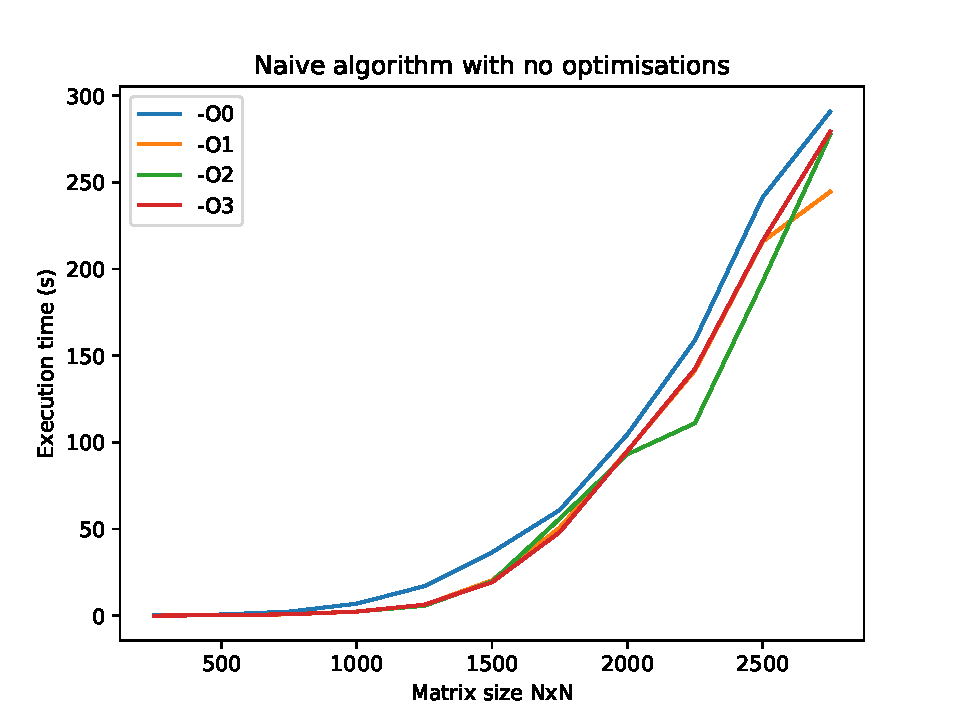
\includegraphics[width=\linewidth]{plot/no_opt.pdf}
    \caption{Naive algorithm performance results}
    \label{fig:no_opt}
\end{figure}

\subsection{Loop nest optimisations}
Here we have a more optimized version \cite{dataloc:1} \cite{looptil:1}
\cite{looptilpar:1},  with many optimisation techniques used:
\begin{lstlisting}
int ib = 10, kb = 10;
for (ii = 0; ii < N; ii += ib) {
    for (kk = 0; kk < N; kk += kb) {
        for (j=0; j < N; j += 2) {
            for(i = ii; i < ii + ib; i += 2 ) {
                if (kk == 0)
                acc00 = acc01 = acc10 = acc11 = 0;
                else {
                    acc00 = res[i + 0][j + 0];
                    acc01 = res[i + 0][j + 1];
                    acc10 = res[i + 1][j + 0];
                    acc11 = res[i + 1][j + 1];
                }
                for (k = kk; k < kk + kb; k++) {
                    acc00 += b[k][j + 0] * a[i + 0][k];
                    acc01 += b[k][j + 1] * a[i + 0][k];
                    acc10 += b[k][j + 0] * a[i + 1][k];
                    acc11 += b[k][j + 1] * a[i + 1][k];
                }
                res[i + 0][j + 0] = acc00;
                res[i + 0][j + 1] = acc01;
                res[i + 1][j + 0] = acc10;
                res[i + 1][j + 1] = acc11;
            }
        }
    }
}
\end{lstlisting}
The first technique used here is register level tiling, which is why we see
four different accumulators, and by doing this we reuse every loaded value from
matrices $a$ and $b$ twice. which reduces the amount of memory loads
necessary.\\

Next we have the $i$ loop blocking. And by blocking we mean the addition of
a second loop ($ii$ loop) that takes larger steps ($ib$) while keeping the
original loop to go through the gaps left by the bigger loop. this technique is
used to increase the locality of the data since we are parsing each matrix in
rectangular strips. We also have the $k$ loop blocked by a factor ($kb$) which
means we'll be parsing the matrices in square strips of sizes $ib$x$kb$, this
will have a major impact on the performance since each square will be reused
multiple times, which reduces the amount of memory loads necessary
significantly. These loop blocks require some further treatment in order for
it to function correctly, for example here we need to explicitly tell it to
initialize the accumulators at $kk==0$ because we aren't viewing the values
contiguously. There are some more special cases that have been omitted from
here that make the code work for values of $N$ that aren't multiples of $ib$
and $kb$.\\

And here we can see some major performance improvements over the naive version.
as well as the fact that these techniques depend heavily on the eventual
compiler's optimisations, because the performance spikes on when the compiler
optimisations are turned off (optimisation level -O0).

\begin{figure}[H]
    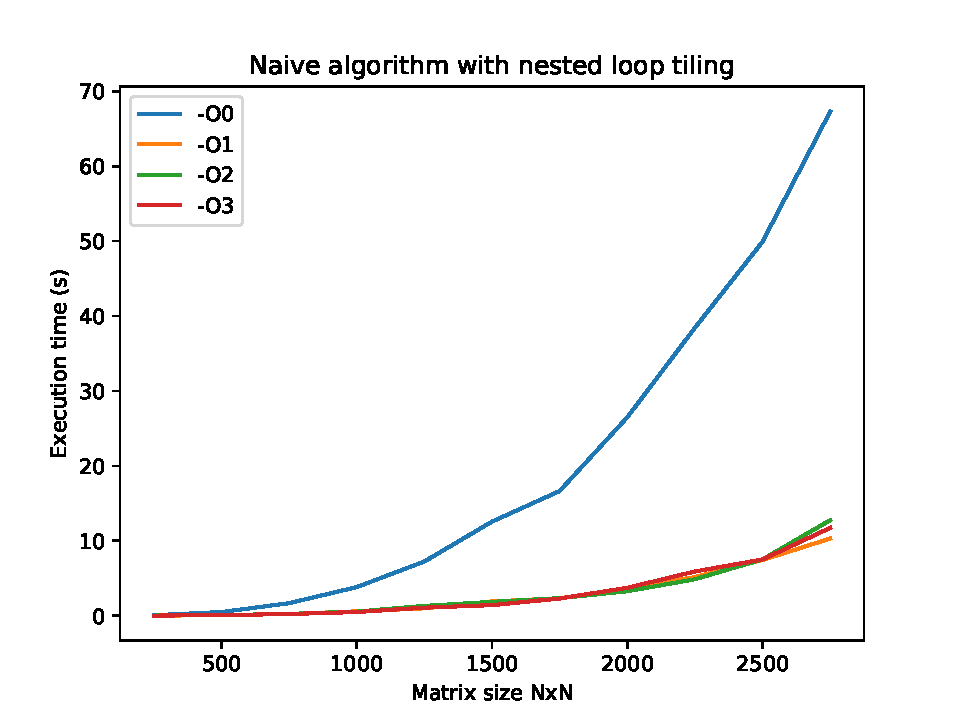
\includegraphics[width=\linewidth]{plot/with_opt.pdf}
    \caption{with register tiling and loop blocking}
    \label{fig:with_opt}
\end{figure}

\subsection{Parallelization}
Here we can see the OpenMP syntax, and we can notice that OpenMP works with C's
pragma directives, the 'omp' part is to specify the OpenMP directives, and
'parallel for' is to say that the next for loop needs to be run in parallel,
next we specify the variables that should be either shared or made private, to
avoid data racing, and we also have the scheduling method for the
parallelization, which in this case is static, meaning the loop's iterations
will be distributed uniformly between the treads.

\begin{lstlisting}
#pragma omp parallel for shared(a, b, res) \\
                         private(i, j, x, acc) \\
                         schedule(static)
for(i=0; i<N; i++) {
    for(j=0; j<N; j++) { 
       acc = 0.0;
       for(x=0; x<N; x++) {
           acc += a[i][x] * b[x][j];
       }
       res[i][j] = acc;
    }
}
\end{lstlisting}

And as visible in the graph, there is a 4 time increase in performance as
expected from a 4 core machine.
\begin{figure}[H]
    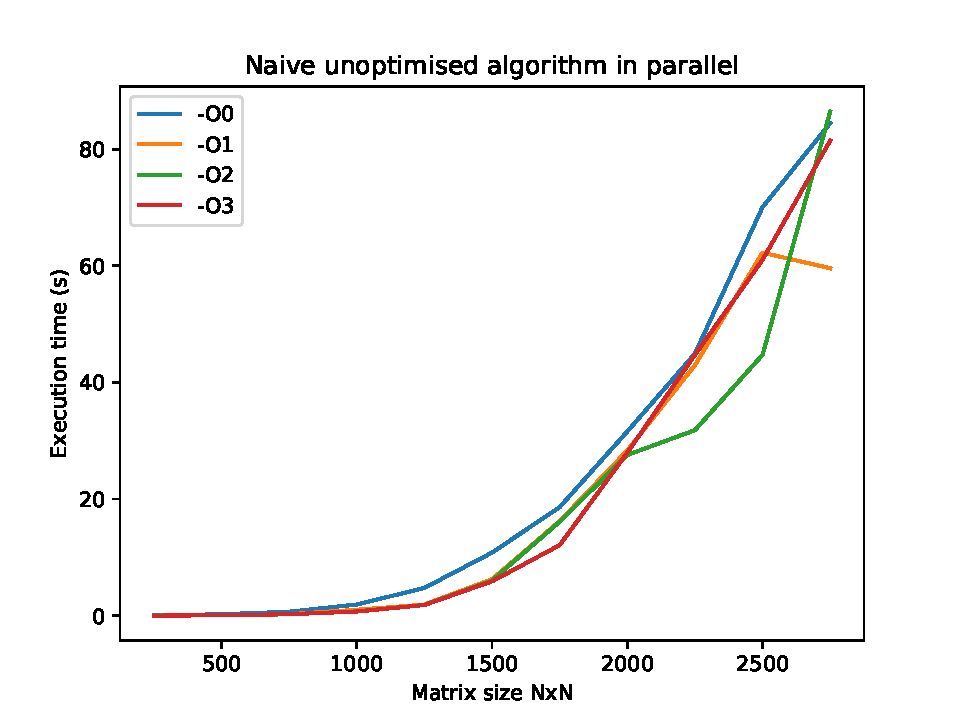
\includegraphics[width=\linewidth]{plot/parallel.pdf}
    \caption{With OpenMP parallelization}
    \label{fig:parallel}
\end{figure}

\subsection{Parallelization and optimisations}
Here we have both the parallel part and optimisation techniques.

\begin{lstlisting}
int ib = 10, kb = 10;
#pragma omp parallel for shared(a, b, res, ib, kb) \\
              private(i, ii, j, k, kk, acc00, acc01, acc10, acc11) \\
              schedule(static)
for (ii = 0; ii < N; ii += ib) {
    for (kk = 0; kk < N; kk += kb) {
        for (j=0; j < N; j += 2) {
            for(i = ii; i < ii + ib; i += 2 ) {
                if (kk == 0)
                    acc00 = acc01 = acc10 = acc11 = 0;
                else {
                    acc00 = res[i + 0][j + 0];
                    acc01 = res[i + 0][j + 1];
                    acc10 = res[i + 1][j + 0];
                    acc11 = res[i + 1][j + 1];
                }
                for (k = kk; k < kk + kb; k++) {
                    acc00 += b[k][j + 0] * a[i + 0][k];
                    acc01 += b[k][j + 1] * a[i + 0][k];
                    acc10 += b[k][j + 0] * a[i + 1][k];
                    acc11 += b[k][j + 1] * a[i + 1][k];
                }
                res[i + 0][j + 0] = acc00;
                res[i + 0][j + 1] = acc01;
                res[i + 1][j + 0] = acc10;
                res[i + 1][j + 1] = acc11;
            }
        }
    }
}
\end{lstlisting}

And we can see that the optimisation techniques scale up with the
parallelization, which implies that there are no bottlenecks.

\begin{figure}[H]
    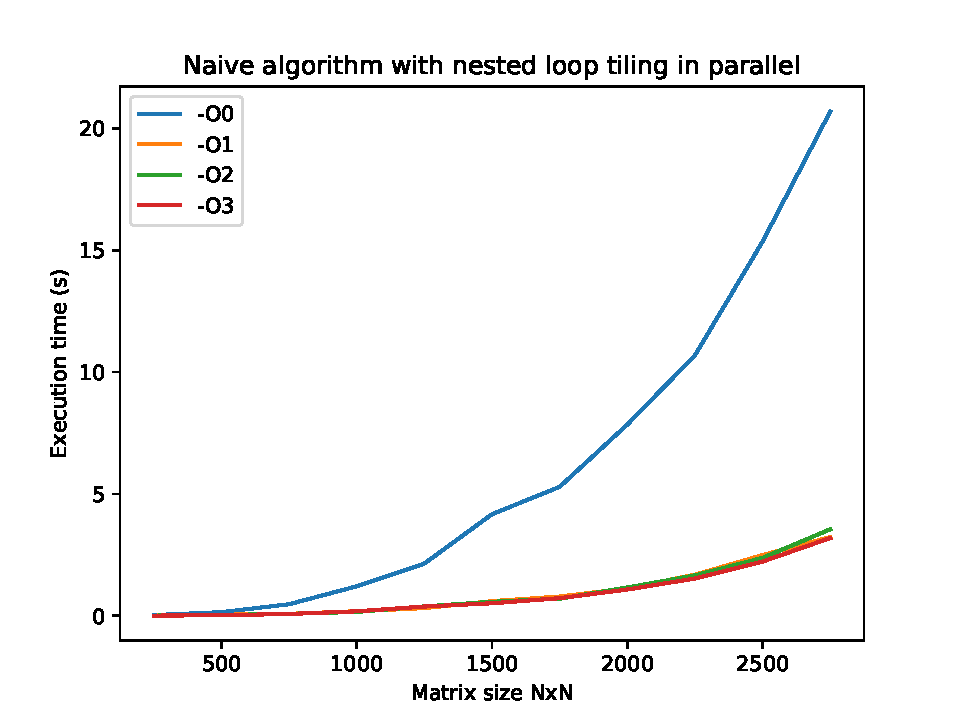
\includegraphics[width=\linewidth]{plot/with_opt+parallel.pdf}
    \caption{With the optimisation and in parallel}
    \label{fig:with_opt+parallel}
\end{figure}

\section{Algorithm comparison}
Here we compare the four different programs on different compiler optimisation
levels.
\begin{figure}[H]
    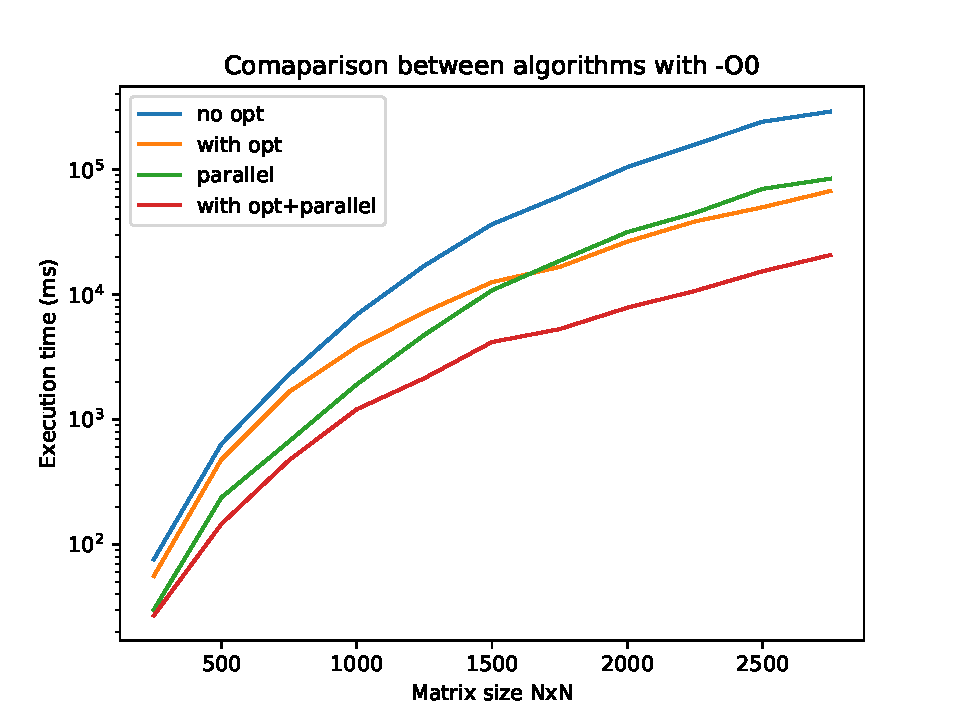
\includegraphics[width=\linewidth]{plot/compare_O0.pdf}
    \caption{comparison with GCC -O0 (on a logarithmic scale)}
    \label{fig:compare_O0}
\end{figure}

\begin{figure}[H]
    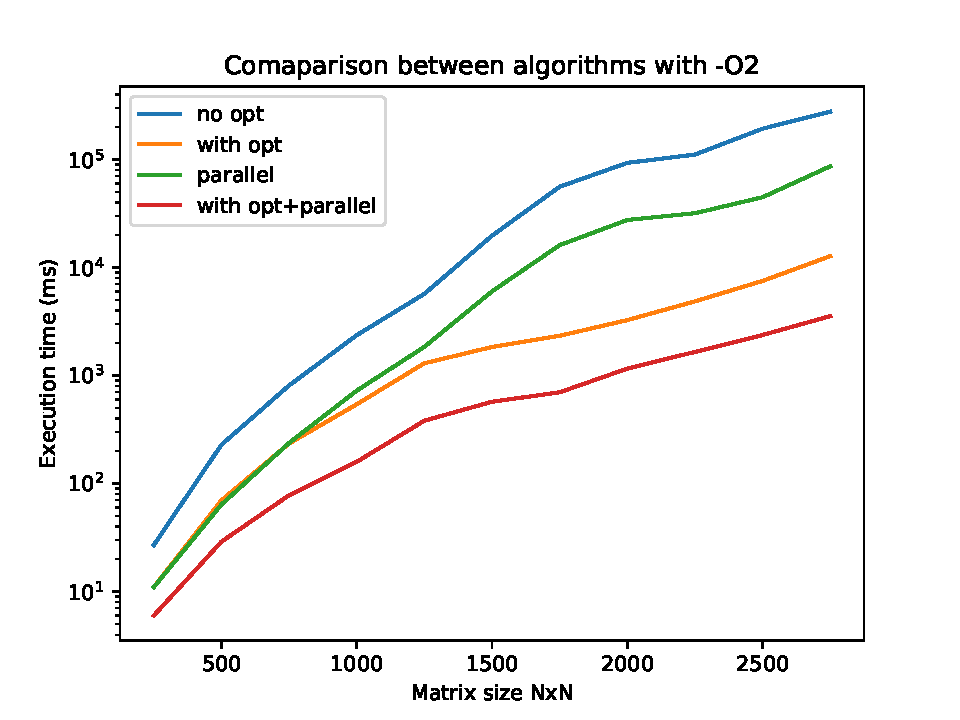
\includegraphics[width=\linewidth]{plot/compare_O2.pdf}
    \caption{comparison with GCC -O2 (on a logarithmic scale)}
    \label{fig:compare_O2}
\end{figure}

We can notice that the parallel naive version is less affected by the compiler
optimisation level, and the loop tiling has a better performance than just
direct parallelization of the code, and of course the combination of the two
gives a major performance improvement.

\section{Code analysis}
With the goal of optimizing the neural network simulator promethe, I started by
trying to parallelize parts of the code using OpenMP, after setting up the
necessary compiler flags and libraries for OpenMP.\\

To benchmark the performance I set up a simple simulation with a hebbian NN
and a noise function as an input, along with a function to measure the elapsed
time of each update (f\_display\_framerate).\\

The first bit of code was in prom\_user/src/main.c where I set up OpenMP to run
the procedure responsible for launching the update functions of the neural
networks in parallel, and here the performance didn't scale up with the
number of threads (with 4 threads ~20\% improvement).\\

After thorough examination of the function reponsible for updating the
neurons's coefficients, which performed a dot product of the neurons
coefficients with their outputs. The problem appeared to come from the memory
access to the neurons coefficients, after a simple test using a simpler 2d
array as a replacement for the coefficients' values. the problem seemed to be
fixed along with a much better execution time.\\

To analyze the cause of this problem I did some research on the subject where
it turned out that the problem was caused by the size of the coefficients structure
(type\_coeff)which was 56 bytes long, this size made it so that each memory
access operation had to be retrieved from the main memory (as opposed to the
cache) at each request from the inner (calcule\_produit) loop. that is, the
entire values were loaded into the cache because the structure took up almost
all of the cache line (usually 64 bytes), that meant that most memory accesses
missed the cache since only about only one element was loaded from the
coefficients array every time. which caused a bottleneck that encumbered the
parallelization because each thread has to wait for the other threads' memory
requests.

\section{Cause of the problem}
To track down the source of the problem, that is, what is causing the
coefficient's structure (type\_coeff) to throttle the performance.
We are going to see basic a overview of how the cache and cache lines work, and
how data is loaded into it.

\subsection{The cache memory}
The cache is a hardware component usually located in the CPU that allows much
faster access times to memory at the expense of the storage size.\\

The main different between the cache and the main memory are the cells that
construct them, where the cache cells are called SRAM, as opposed to the DRAM
cells in the main memory.\\

In modern CPUs there are multiple levels (typically 3, L1, L2 and L3) of cache
where L1 is a few tens of KBs, and L2 a few hundreds of KBs, and the third level
a few MBs, and the first level is usually much faster than the second which in
turn is faster than the third, all of which are faster than the main
memory (Figure:\ref{fig:compram}).

\begin{figure}[H]
    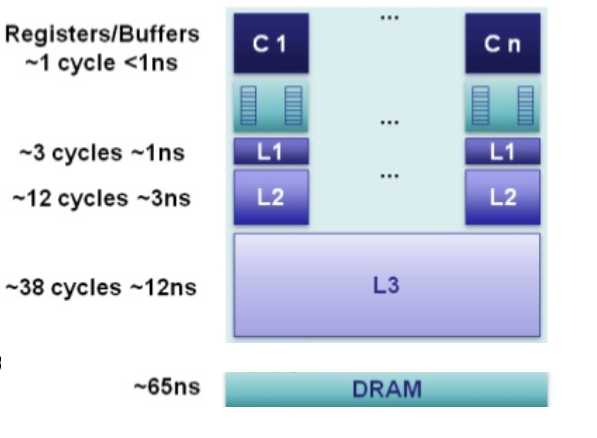
\includegraphics[width=\linewidth]{plot/cacheperf.png}
    \caption{Speed of the different levels of cache and DRAM}
    \label{fig:compram}
\end{figure}

When accessing some data from the memory, the L1 cache is first checked for and
if it had been previously loaded there we can utilize the L1's fast access time
to get the data, and we call that a \textbf{cache hit}, and when we don't find the
wanted data in it we call it a \textbf{cache miss} instead.\\

If there was a cache miss on the L1 cache we try the L2, and if that misses we
try the L3 and then we finally try the main memory (DRAM) if even that misses.

\subsubsection{DRAM vs SRAM}
The dynamic random-access memory (DRAM) and static random-access memory (SRAM)
cells differ on an architectural level (Figure:\ref{fig:dramsram}), where each 
cell of the SRAM is constructed of 6 cleverly placed transistors. Whereas the DRAM
uses a single transistor and a capacitor, the capacitor in where the actual bit of
data is stored which is the cause of slow access time since the capacitor needs
to be completely depleted in order to read the bit value stored, and considering
the size of the capacitors here the capacitor discharges automatically with
time,which adds the requirement for a constant refresh of the cells to recharge
the cells, this usually happens every 64ms and is also part of the reason the
DRAM is slower. \cite{dramsram:1}

\begin{figure}[H]
    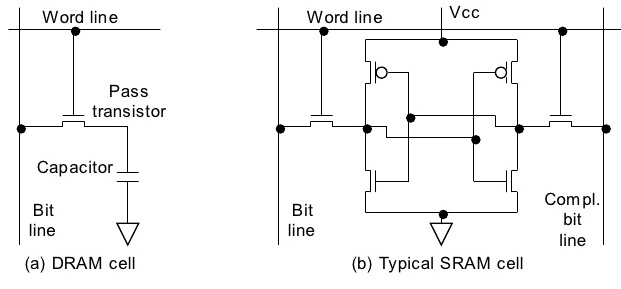
\includegraphics[width=\linewidth]{plot/dram_sram.jpg}
    \caption{Cell architecture of DRAM and SRAM}
    \label{fig:dramsram}
\end{figure}

\subsubsection{Cache lines}
Cache lines are the smallest block of memory that we can access \textit{i.e.}
load into the cache, they are usually 64 bytes or 32 bytes \ref{fig:cachelines}
the idea is that if we even load a single byte from the memory, the entire
cache line that byte belongs to is loaded into the cache. Meaning if we try
to access the byte right after it in memory (which is most probably the case)
we can simply retrieve it from the cache instead.\\

The cache line is the same for all different levels of the cache, what changes
however is of course how fast the memory level gets filled, the first level
having the least amount of storage usually fills up first and so we have less
L1 hits than L2 or L3 overall.\\

\begin{figure}[H]
    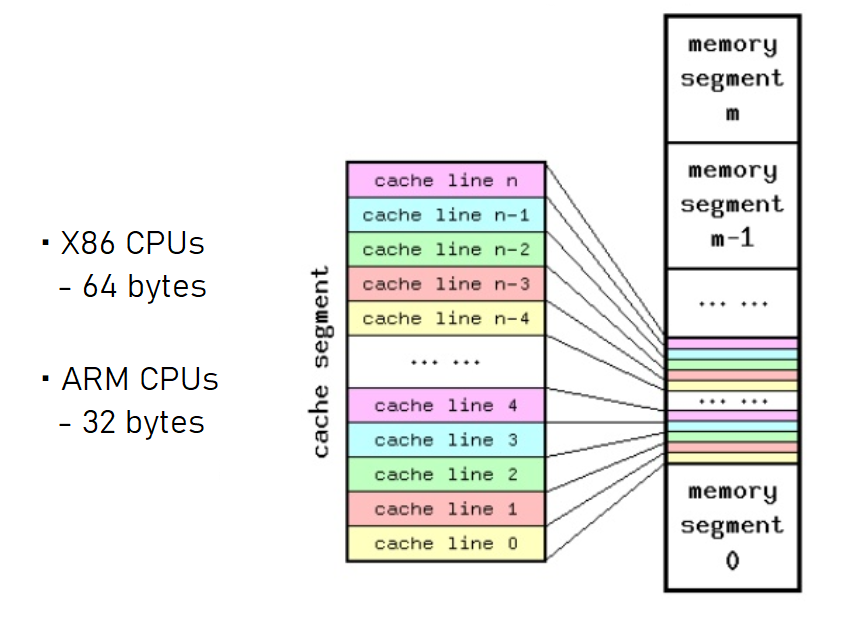
\includegraphics[width=\linewidth]{plot/cachelines.png}
    \caption{Memory cache lines}
    \label{fig:cachelines}
\end{figure}


\subsubsection{The cause}
From we can already see that the use of an array of the (type\_coeff) with
a size of 56 bytes would fill almost the entirety of the cache line
\ref{fig:cachedist}, meaning overall we'll have almost no cache hits, even if
we access the coefficients array elements contigously (\textit{ex:} coeff[0]
then coeff[1] then coeff[2] and so on).

\begin{figure}[H]
    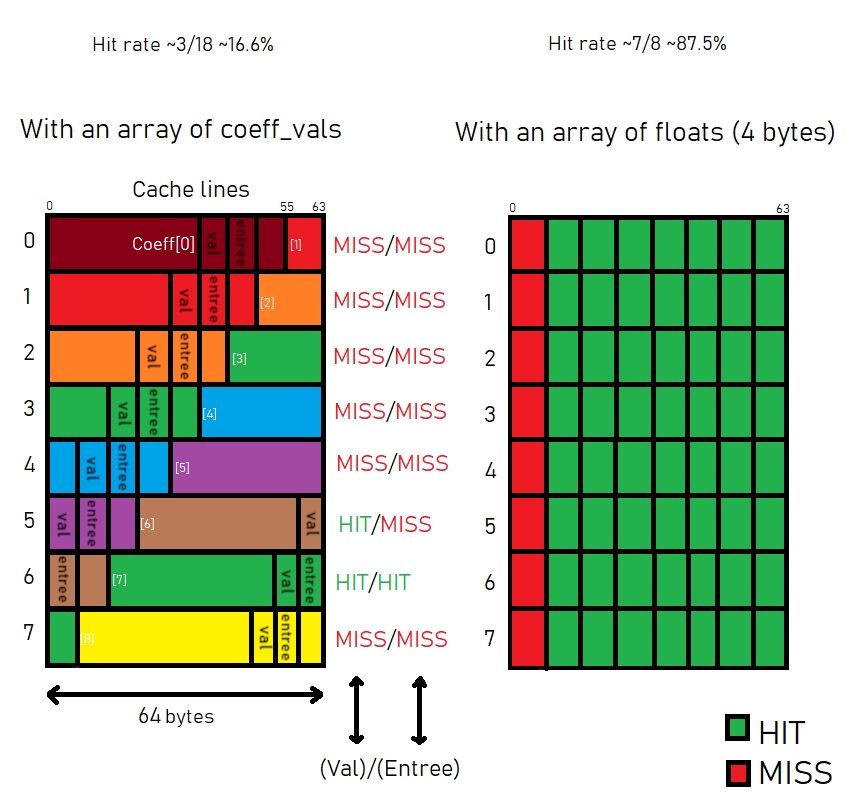
\includegraphics[width=\linewidth]{plot/cachedistr.png}
    \caption{Cache hits on an array of type\_coeff and another of floats}
    \label{fig:cachedist}
\end{figure}

All of this would mean we would barely be using the cache (16.6\% hit rate)
and the computations will be dependent on the main memory's DRAM. which
completely throttles the CPUs calculations since a since an access to the DRAM
takes tens of clock cycles (Figure:\ref{fig:dramsram}).\\

This here constitutes a bottleneck that has to be resolved before trying to
parallelize the code, and it also explains the insignificant improvement from
parallelizing the code previously where there was only a 20\% performance
increase on a 4 core machine, where it should have been 4 times faster.

\section{Solution and results}
Ideally the best solution would be to turn all the fields of the type\_coeff 
structure into arrays, and also we would also need to remove the s field that
references the next coefficient.
\begin{lstlisting}[numbers=none,frame=none,xleftmargin=3em, multicols=2]
OLD STRUCT:

typedef struct type_coeff {
  float val;
  float proba;
  float Nbre_ES;
  float Nbre_S;
  float Nbre_E;
  int entree;
  int type;
  int evolution;
  float moy;
  float smoy;
  int gpe_liaison;
  struct type_coeff *s;
} type_coeff;
NEW STRUCT:

typedef struct type_coeff {
  float *val;
  float *proba;
  float *Nbre_ES;
  float *Nbre_S;
  float *Nbre_E;
  int *entree;
  int *type;
  int *evolution;
  float *moy;
  float *smoy;
  int *gpe_liaison;
} type_coeff;
\end{lstlisting}

And we would also need to change the type\_neuron structure to have a single
element of type\_coeff (instead of a pointer):
\begin{lstlisting}[numbers=none,frame=none,xleftmargin=3em, multicols=2]
OLD STRUCT:

typedef struct type_neuron {
   float seuil;
	int flag;
	float last_activation;
	float cste;
	int groupe;
	int nbre_voie;
	int nbre_coeff;
	int nbre_coeff_neuromod;
	char max;
	float posx;
	float posy;
	float posz;
	type_coeff *coeff;    ---->
	type_coeff *nsor;     ---->
} type_neuron;
NEW STRUCT:

typedef struct type_neuron {
   float seuil;
	int flag;
	float last_activation;
	float cste;
	int groupe;
	int nbre_voie;
	int nbre_coeff;
	int nbre_coeff_neuromod;
	char max;
	float posx;
	float posy;
	float posz;
	type_coeff coeff;
	type_coeff nsor;
} type_neuron;

\end{lstlisting}

This of course is a major architectural change and would require a lot of other
changes and adjustments to the code base, especially the deletion of the s field 
from the type\_coeff.\\

So instead, for now, in order to benchmark the impact of a similar change on
the code, two float matrices for the 'val' and 'entree' (named respectively
coeff\_vals and coeff\_entrees) fields of the coefficients
were used instead, and were initialized and updated with the same values as the
actual values from the type\_coeff structure. The changes are limited to the
hebbian neural network (prom\_user/src/NN\_Core/classique\_rn/trad\_neuron.c)
and the kohonen self-organizing map (same directory in kohonen.c). and the
results seem to reflect that the changes solved the bottleneck and the code can
run in parallel (Figure:\ref{fig:hebbres}) (Figure:\ref{fig:kohonenres}). 

\begin{figure}[h]
    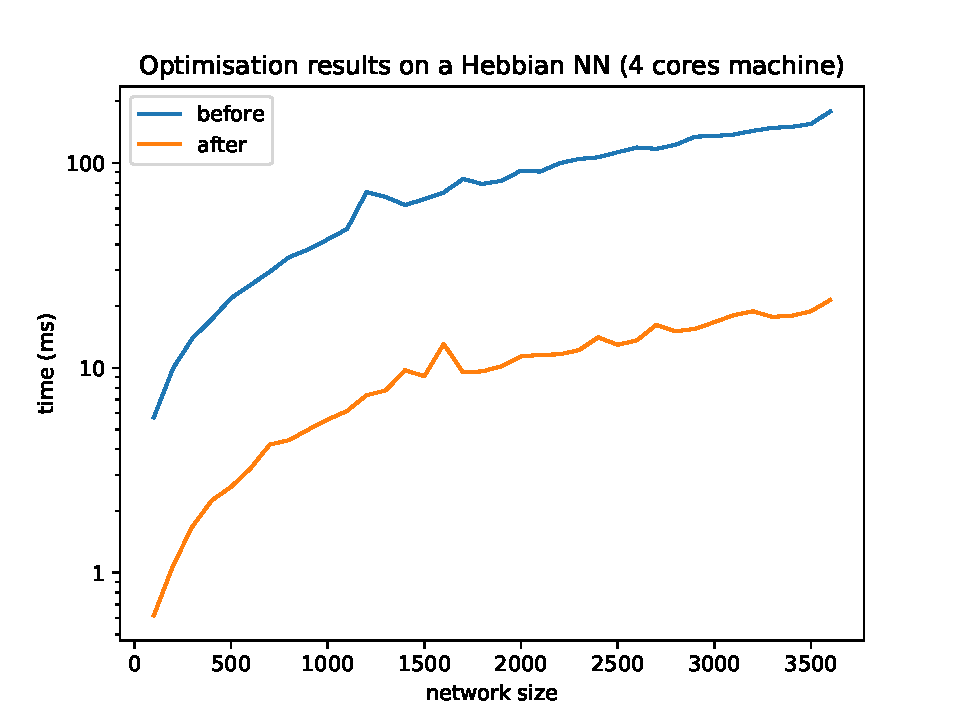
\includegraphics[width=\linewidth]{plot/hebbres.pdf}
    \caption{Results of the optimisation on hebbian NN}
    \label{fig:hebbres}
\end{figure}

\subsection{tests}
To verify that the program continues to function correctly some tests were created
that compare results (coefficient values) of the original version of the program
(without the optimisation) with the new version.\\

In order to do this the two versions of the program  were used to compile a test
.script file with their cc\_leto (used to generate a .res file used when
executing the promethe simulator) that prompts for a seed for the random number
generator, these programs when launched (using promethe) generate a .SAVE file
that contains a text version of the coefficients and their values. The idea of
the test is that given the same random seed, these two .SAVE files should be
the same for the two versions.

For now these tests still need some more work done on them since they are not
working. There is still a lot of work to be done here in order to utilize the new
optimisation and there's the question of how much more \textit{should} be done, 
since these are major changes to a very large code base, and would therefore
require a lot of time to implement.

\begin{figure}[H]
    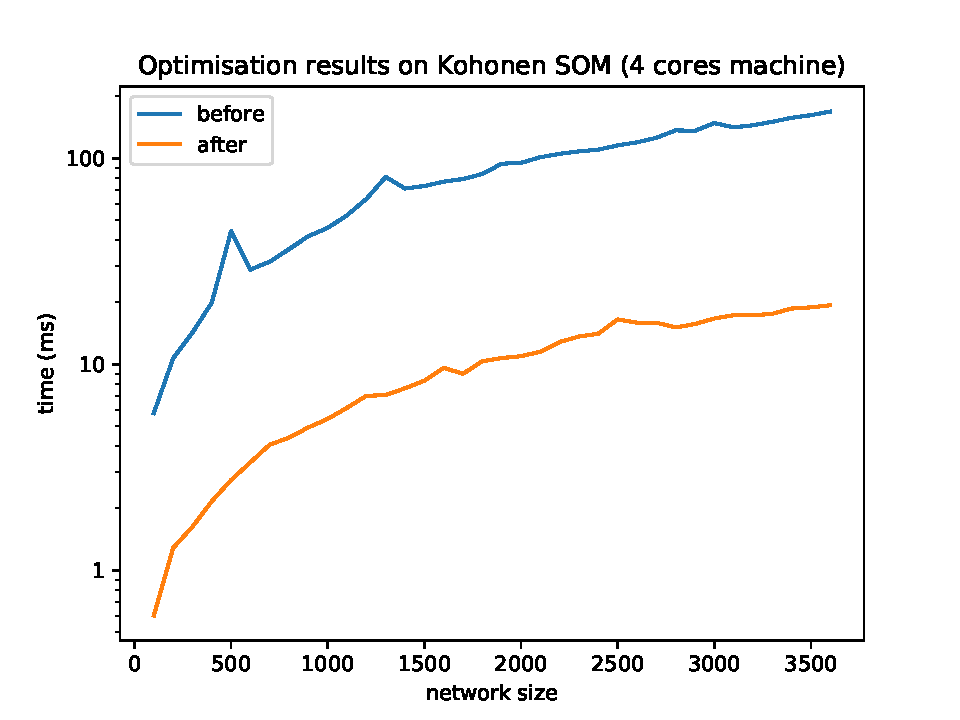
\includegraphics[width=\linewidth]{plot/kohonenres.pdf}
    \caption{Results of the optimisation on kohonen SOM}
    \label{fig:kohonenres}
\end{figure}

\section{Conclusion}
It seems that in order to utilize the cache's fast access time, and to avoid
memory access bottlenecks. The data needs to be divided into contiguous arrays
of small chunks (few bytes, float for example) of the same field (for example 'val')
this makes sure that cache lines will contain more of these small chunks as opposed
to having an array of a big structure (tens of bytes) which would cause the
cache lines to only one or two copies of the structure, plummeting the hit rate
on the cache.\\

This is a result of the fact that we only use a few fields of the structure at
any given time (we only use the 'val' and 'entree' fields when updating hebbian
NN neurons), so most of the cache line is not used and wasted. However when there
are multiple arrays of each field (floats) or small collection of
fields, we would have more elements of the same type in our cache lines and
therefore more hits of accelerated memory access of the CPU's cache.

\newpage

\bibliography{bibliography} 
\bibliographystyle{ieeetr}

\end{document}
